%% Use the "review" option when submitting for review.
%% Removing the "review" option will switch the
%% manuscript to a two-column layout.

\documentclass[jog]{igs}

\usepackage[utf8]{inputenc}

\usepackage{mathabx}
\usepackage{graphicx}
\usepackage{siunitx}

% the default is for unnumbered section heads
% if you really must have numbered sections, remove
% the % from the beginning of the following command
% and insert the level of sections you wish to be
% numbered (up to 4):

% \setcounter{secnumdepth}{2}

\jourvolume{V}
\jourissue{N}
\jourpubyear{YYYY}

\begin{document}

\title[Sankey mass flows]{Ice sheet mass flows}

\author[Mankoff and others]
       {Kenneth D. MANKOFF,$^{1,2}$
         Xavier FETTWEIS,
         Chad GREENE,
         Brice VAN LIEFFERINGE,
         Someone, ELSE,$^n$,
       add your name to CREDIT.CSV in repository}

\affiliation{%
  $^1$NASA Goddard Institute for Space Studies, New York, NY, 10025 USA\\
  $^2$Autonomic Integra LLC, New York, NY, 10025 USA\\
  $^n$Somewhere Else\\
  Correspondence: Ken Mankoff
  \email{ken.mankoff@nasa.gov}}

\begin{frontmatter}
\maketitle
\begin{abstract}

  Understanding the processes involved in ice sheet mass loss requires knowledge production and sharing, in addition to field observations and computer modeling. Tabular data is optimized for computers and useful for humans, but graphical presentations can provide significantly higher information density. Here we present several Sankey diagrams depicting all mass flow of water in various phases in Greenland and Antarctica. Sankey diagrams help bring perspective to the interplay and relative importance of snowfall, rain, drawdown, refreezing, submarine melt, iceberg calving, and grounding line retreat in contributing to ice sheet mass balance.

  This work quantifies both grounded and floating ice mass loss. From this, mass loss in Greenland is 330 Gt yr$^{-1}$ which is \(\sim\)25 \% higher than the \(\sim\)270 Gt yr$^{-1}$ estimates that neglect terminus retreat of ice at or near flotation. Mass loss in Antarctica is 275 Gt yr$^{-1}$ which is \(\sim\)85 \% higher than the \(\sim\)150 Gt yr$^{-1}$ estimates of grounded ice mass loss.

  This work also reports gross not net values, which is useful for example for quantifying total freshwater export from an ice sheet. For example, freshwater export due to frontal retreat is not 60 Gt yr$^{-1}$, but rather nearly six times larger at 345 Gt yr$^{-1}$ due to 345 Gt yr$^{-1}$ of frontal retreat offset by 285 Gt yr$^{-1}$ of frontal advance, with the difference as the commonly reported value of 60 Gt yr$^{-1}$.
\end{abstract}
\end{frontmatter}

\section{Introduction and Background}

Mass loss from the grounded portion of the Greenlandic and Antarctic ice sheets contributes to sea level rise (SLR), and can be captured by a single value per ice sheet. Reporting a single value is beneficial because it simplifies interpretation and comparison. However, ice sheets are complex systems and while their contribution to sea level rise is important, it is not a holistic view and does not capture the general health and state of the ice sheet. Few studies consider all processes and their relative magnitudes and uncertainties - this is typically limited to review papers, which may not focus on quantitative assessment of each process. As one example, an ice sheet that increases output via discharge or submarine melting by X \% but has that offset by an equal increase in snowfall would report no net mass change or net SLR contribution, but has entered a different state when viewing constituent terms or gross values.

Net mass flow (mass balance) is typically analyzed using one or a combination of three methods. Of these, the gravimetric method cannot observe mass change of floating ice, the volumetric method cannot distinguish between surface and basal processes, and only the input-output method can estimate both mass flow, all processes participating in mass flow, and the subsequent mass change.

Here we present Sankey diagrams that provide an overview of all mass flow terms and processes for both the Greenlandic and Antarctic ice sheets.

% We use this display to highlight a) relative magnitudes among processes within ice sheets and among ice sheets and sectors, and b) the uncertainty associated with each property. We also... TBD.

\begin{figure*}
\centering{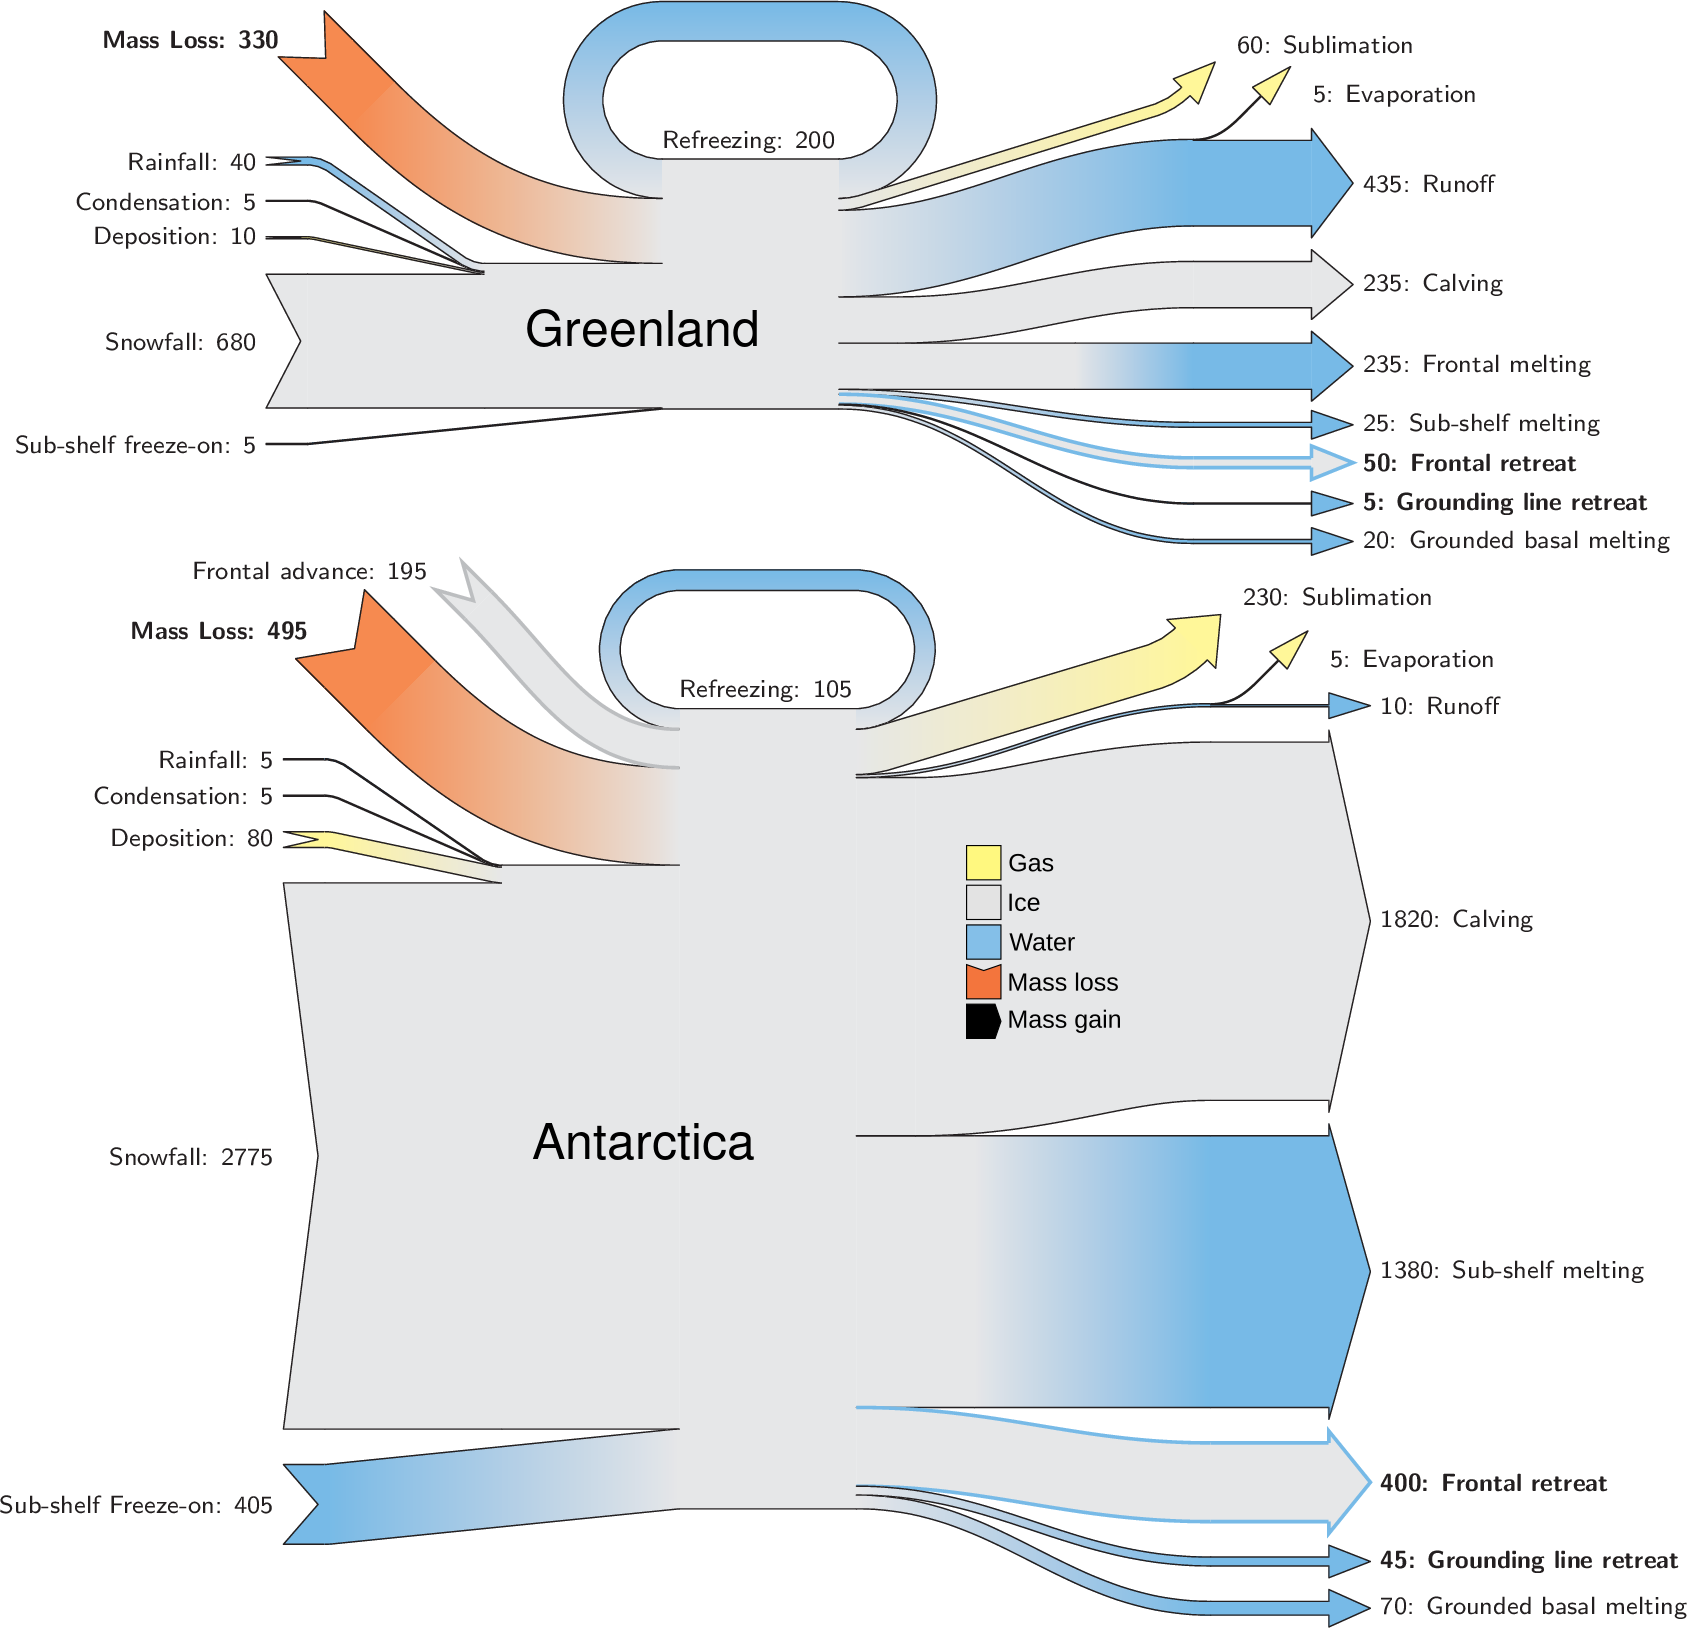
\includegraphics[width=0.85\textwidth]{fig_aq_gl.png}}
\caption{Sankey mass flow diagrams for Antarctica and Greenland, and Antarctica split into East, West, and Peninsula. All widths are proportional within and between images. Because Sankey diagrams balance all inputs and outputs, mass losses require a `drawdown' input (red) to balance the larger outputs, and mass gains requires an `accumulation' output (black) to balance the larger inputs.}
\label{fig}
\end{figure*}

\subsection{Introduction to Sankey diagrams}

Sankey diagrams are graphical representations of flow or movement of any property (e.g., mass, energy, money, etc.). An early and famous use was Charles Minard's Map of Napoleon's Russian Campaign of 1812 (c.f., \citet{kraak_2021}) that combines the magnitude of active soldiers overlaid on a geographical map to show attrition during one battle in a war. The method was later refined, popularized, and eventually named after Captain Matthew Henry Phineas Riall Sankey who used it to show, among other things, the energy efficiency of a steam engine.

A similar display to the diagrams presented here by \citet[Fig. 2]{cogley_2011} shows flows overlaid an a glacier schematic and here we build on that work by adding magnitude of processes and making the graphics proportional to magnitudes.

\section{Methods}

We use a combination of existing published values, new estimates, and derived values.

Existing published values include 

The derived value is only the net mass change - here shown as `drawdown' in Greenland and West Antarctica, or `accumulation' in Antarctica, East Antarctica, or the Peninsula (Fig \ref{fig}). This term balances all the other terms, so that the Sankey diagram has outputs balancing inputs.

In Greenland, there is no known assessment of grounding line retreat separate from ice front retreat. These two terms are the same in most places in Greenland, because there are few ice shelves. In these locations, we used published values from \citet{kochtitzky_2023} and assign this to frontal retreat. There are published values of grounding line retreat at some glaciers, but units are typically m and not Gt yr$^{-1}$. Here we use published values of Petermann glacier grounding line retreat (units m) from \citet{millan_2022}, ice velocity from \citet{millan_2022}, ice thickness from \citet{ciraci_2023}, and an estimate of ice density of 917 kg m$^{3}$ to calculate grounding line retreat in units of Gt yr$^{-1}$. We estimate \sim 1.5 Gt yr$^{-1}$, and round this up to 5 Gt yr$^{-1}$ to account for all other ice shelf grounding line retreat in Greenland.

Condensation: TODO

Deposition: TODO

In Antarctica, we use the MEaSUREs Antarctic Boundaries for IPY 2007-2009 from Satellite Radar, Version 2 (NSIDC product 0709; \citet{mouginot_2017,rignot_2013}) to separate Antarctica into East, West, and Peninsula. We drop all unattached islands, so the sum of the regional terms may not equal the total Antarctic values in Fig. \ref{fig}.

\subsection{Sankey diagrams}

The Sankey diagrams shown here are generated from a script that combines a CSV file of values with a \LaTeX\ template that uses the TikZ Sankey package \citep{sankey}. This architecture makes it trivial to generate similar diagrams for other time periods, differences between time periods, after generating CSV files with representative values. 

\section{Missing terms and limitations}
\label{sec:limits}

These figures neglect some mass flow processes (some of which are included in \citet[Fig. 2]{cogley_2011}), and simplify others.

Neglected processes include basal freeze-on (e.g., \citet{bell_2014}). It is currently unknown by Ken (TODO: Nanna,  Brice?) if this is refreezing of the basal melting term (i.e., \citet{karlsson_2021} Greenland and \citet{pattyn_2010} Antarctica) and therefore that source remains unchanged, but some diverts back to the dynamics flow and the basal melting output is reduced, or if the basal melting term is final basal runoff, in which case the source should be increased by the refreezing amount. Nonetheless, we do not yet know nor estimate the refreezing magnitude.

We also neglect avalanche on and off - these likely matter more for mountain glaciers than ice sheets.

Snow drift on and off is also excluded. There is likely little snow drift onto either ice sheets, but drifting off may be of similar magnitude to other terms. Some drift off may be implicitly included in the sublimation term (TODO: Xavier?)

There may be other missing terms. For example, the earlier version of this graphic by \citet[Fig. 2]{cogley_2011} did not contain frontal nor grounding line retreat. These are two distinct processes when ice shelves exist, but can be treated as synonyms for one process at tidewater glacier margins. These terms were not only not included in \citet{cogley_2011}, but their respective values were highly uncertain, and still are, although recent work by \citet{kochtitzky_2023,greene_2024} have constrained these values in Greenland. 

We make the following simplifications.

Subaerial frontal melt and sublimation (the vertical face in above the water line, \citet[Fig. 2]{cogley_2011}) is not explicitly treated but is included in other terms.

There are a variety of other simplifications. For example, rainfall input does not all turn to ice. Some enters as part of the refreezing loop, and some remains liquid and leaves as runoff or evaporation. Similarly, the evaporation output could pull from the refreezing loop (in the liquid phase, depicted by the blue color) and also directly from rainfall as stated above. Although some path details are simplified, the magnitudes are still correct - at least as well as we are able to estimate them.

\section{Uncertainty}

Note that some uncertainty (e.g. snowfall) is larger than many other terms combined.

Advice from Hester: Synthesize what each of the uncertainties is a function of (lack of measurements/scale/timing of measurements/lack of process understanding/variability/etc.). Also, rather than singling the uncertainty of each factor the feedbacks between them could be indicated.

This could be the largest section of text.

\section{Comparison with existing estimates}

As previously stated, few existing studies outside of review papers address all terms, and the review papers usually do not focus of quantitative assessment of magnitude. Therefore, we compare parts of this graphic to other existing estimates.

The ice sheet mass balance intercomparison experiment (IMBIE; \citet{otosaka_2023}) reports recent Greenlandic ice sheet mass loss as -257 \pm42 Gt yr$^{-1}$. Elsewhere the gravimetric method reports recent Greenlandic mass loss of ~277 Gt yr$^{-1}$ (GRACE site, need CITATION). These are both significantly less than our estimate of 325 drawdown in order to balance the inputs with outputs. This can be directly attributable to the gravimetric method not observing frontal retreat (50 Gt yr$^{-1}$) nor grounding line retreat (5 Gt yr$^{-1}$). When these loss terms are removed from our estimate, it becomes 270 Gt yr$^{-1}$ which is well within the uncertainty.

In Antarctica...


%% \subsection{Shelves} %% Suggest remove:

%% Mass change of shelves is a bulk aggregate property, and should not the default reporting metric because it obscures information. For example, in theory ice shelf mass can grow even as they collapse, as long as the grounding line retreats (adds mass to the shelf from the upstream ice sheet) faster than the mass loss at the frontal or submarine boundaries. A mass flow diagram dedicated to ice shelves (this one is not) would clearly convey each of these processes. 

%% \subsection{Drifting snow}

%% %% From Hester: I think if you were to go into a discussion of snowdrift it should go further than, for example, the works of Lenaerts et al. Perhaps it is beter to plainly list the uncertainties / poor definitions but in terms of process just refer to the existing papers. However, I am in two minds about this.

\subsection{Interpretation of graphics}

Sankey diagrams are generally intuitive, but the following section may still be helpful in interpreting the diagram(s) shown here. The widths of all lines are proportional to all other widths, both within and among figures. Color here represents both phase and net mass change. Colors gray, blue, and yellow represent solid, liquid, and gaseous phases respectively, while red and black highlight net mass loss or gain. The latter may be counter-intuitive - for example to see mass loss as an input at the top (red in Fig. \ref{fig}) even though most mass loss terms (runoff, calving, etc.) are at the bottom. This is because Sankey diagrams are balanced, outputs are larger than inputs (hence net mass loss), so the mass loss term is an input - drawdown of the historical 'stable' ice mass. Conversely, in East Antarctica mass gain is an output at the bottom (black in Fig. \ref{fig}} that balances the diagram, because without it, there are more flows into the system than out of it.

  These diagrams also do not represent every process perfectly. For example, frontal retreat is a combination of discharge and submarine melting (and should therefore divide between ice and liquid, with the same uncertainty \citep{enderlin_2013}, but frontal retreat is shown separately here because it is usually treated separately in the literature.

  We highlight frontal retreat and grounding line retreat both with a red outline, and by not including frontal retreat in the larger (in Greenland) discharge and submarine melting flow. We do this for two reasons.

  First these two terms imply an imbalance. Regardless of if a system is gaining mass (Antarctica), losing mass (Greenland) or appears to be in steady state (Peninsula), if there is grounding line and frontal retreat, it implies a system imbalance in the long term, even if not a numerical imbalance as represented here.

  Secondly, these two terms are rarely included in mass change estimates. The gravimetric method does not see these processes, the volumetric method is usually cropped at the some fixed grounding line upstream of these processes, and the IO method has typically ignored these two terms as downstream of the flux gates.
  
\section{Acknowledgements}

We thank \citep{sankey} for the \LaTeX\ TikZ Sankey package, and \citet{cogley_2011} for a reference graphic. Analysis was aided by the software packages Pandas (\citet{pandas_team}), Xarray (\citet{xarray}), and GRASS GIS (\citet{GRASS}), among other tools.

We thank Jakob Steiner, Xavier Fettweis, Benjamin Davison, Anna Hogg, Chad Greene, Katie Leonard, Jan Lenaerts, Damien Ringeisen, Liam Colgan, Robert Fausto, Dominik Fahrner, Nanna Karlsson, Brice Van Liefferinge, and Andreas Ahlstrøm for conversations in the development of this work.

\bibliography{library}
\bibliographystyle{igs}

\appendix
\section{Appendix A}
\label{sec:appendix:A}

\begin{table*}
\caption{Mass flow values used for Greenland in Fig. \ref{fig}}
\label{tab:gl}
\begin{tabular}{@{}lcc}\hline
  Term & Source\\
  Snowfall & \citet{fettweis_2020}\\
  Rainfall & \citet{fettweis_2020}\\
  Condensation & TODO\\
  Deposition & TODO\\
  Sublimation & \citet{fettweis_2020}\\
  Evaporation & \citet{fettweis_2020}\\
  Runoff & \citet{fettweis_2020}\\
  Refreezing & \citet{fettweis_2020}\\
  Frontal retreat & \citet{kochtitzky_2023,greene_2024}\\
  Grounding line retreat & Estimated here\\
  Discharge + submarine melting & \citet{mankoff_2020_solid}\\
  Split of discharge \& submarine melting & \citet{enderlin_2013}\\
  Basal melting & \citet{karlsson_2021}\\
  Drawdown & Derived from above terms
\end{tabular}
\end{table*}

\begin{table*}
\caption{Mass flow values used for Antarctica and Antarctica regions in Fig. \ref{fig}}
\label{tab:aq}
\begin{tabular}{@{}lcc}\hline
  Term & Source\\
  Snowfall & \citet{fettweis_2020}\\
  Rainfall & \citet{fettweis_2020}\\
  Condensation & TODO\\
  Deposition & TODO\\
  Sublimation & \citet{fettweis_2020}\\
  Evaporation & \citet{fettweis_2020}\\
  Runoff & \citet{fettweis_2020}\\
  Refreezing & \citet{fettweis_2020}\\
  Frontal retreat & TODO\\
  Grounding line retreat & TODO\\
  Discharge + submarine melting & \citet{davison_2023}\\
  Split of discharge \& submarine melting & \citet{davison_2023}\\
  Basal melting & \citet{van-liefferinge_2013}\\
  Drawdown or accumulation & Derived from above
\end{tabular}
\end{table*}

\section{Appendix B}
\label{sec:appendix:B}

\begin{figure*}
\centering{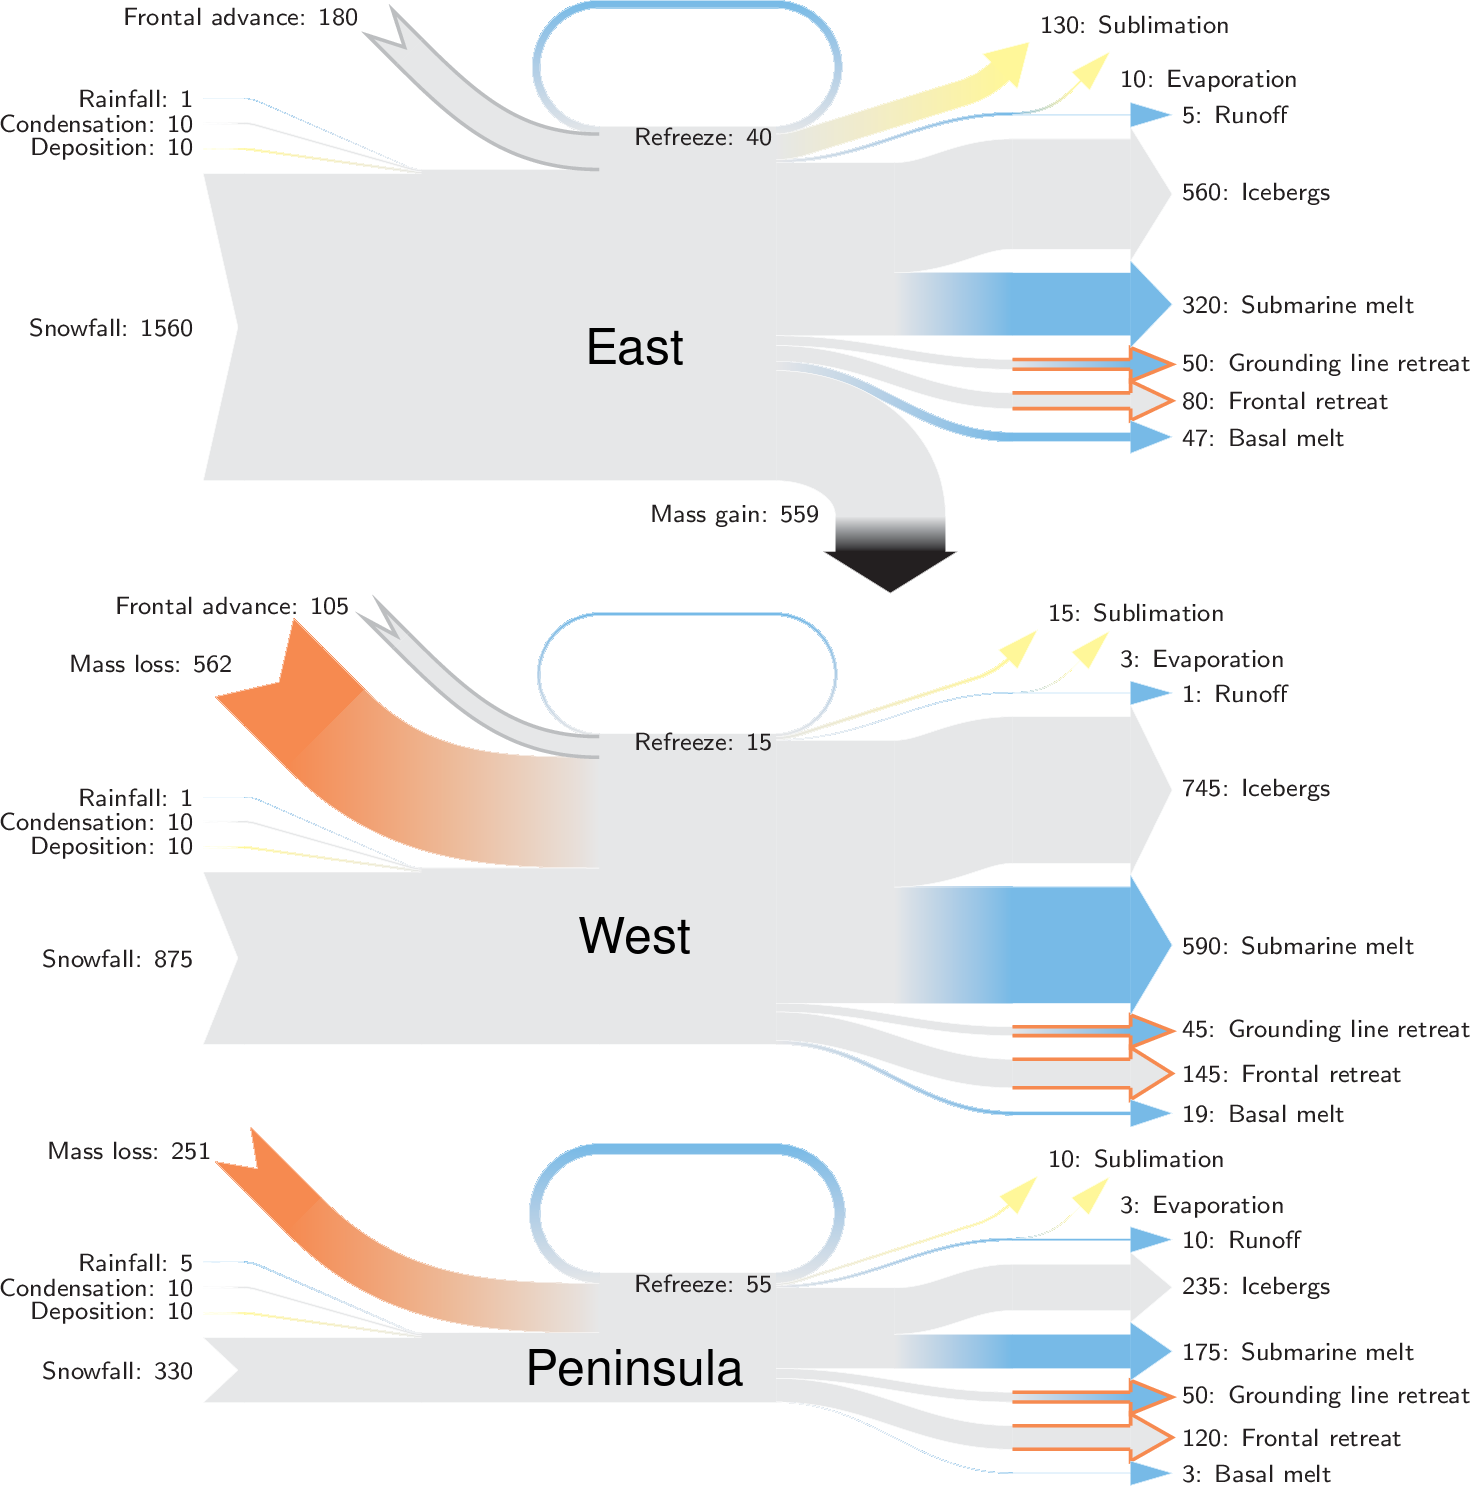
\includegraphics[width=0.85\textwidth]{fig_aq_parts.png}}
\caption{Sankey mass flow diagrams for Antarctica and Greenland, and Antarctica split into East, West, and Peninsula. All widths are proportional within and between images. Because Sankey diagrams balance all inputs and outputs, mass losses require a `drawdown' input (red) to balance the larger outputs, and mass gains requires an `accumulation' output (black) to balance the larger inputs.}
\label{fig}
\end{figure*}

\end{document}
